% Standalone RAKL capstone diagram (Paper VI, Figure: four coupled loops + authority firewall).
% Build:  pdflatex four_loop_master.tex  -> four_loop_master.pdf
\documentclass[border=6pt]{standalone}
\usepackage{tikz}
\usepackage{amsmath}
\usepackage{helvet}\renewcommand{\familydefault}{\sfdefault}
\usetikzlibrary{positioning,arrows.meta,shapes.geometric,fit,backgrounds,calc}
\definecolor{oiblue}{HTML}{0072B2}
\definecolor{oiverm}{HTML}{D55E00}
\definecolor{oigreen}{HTML}{009E73}
\begin{document}
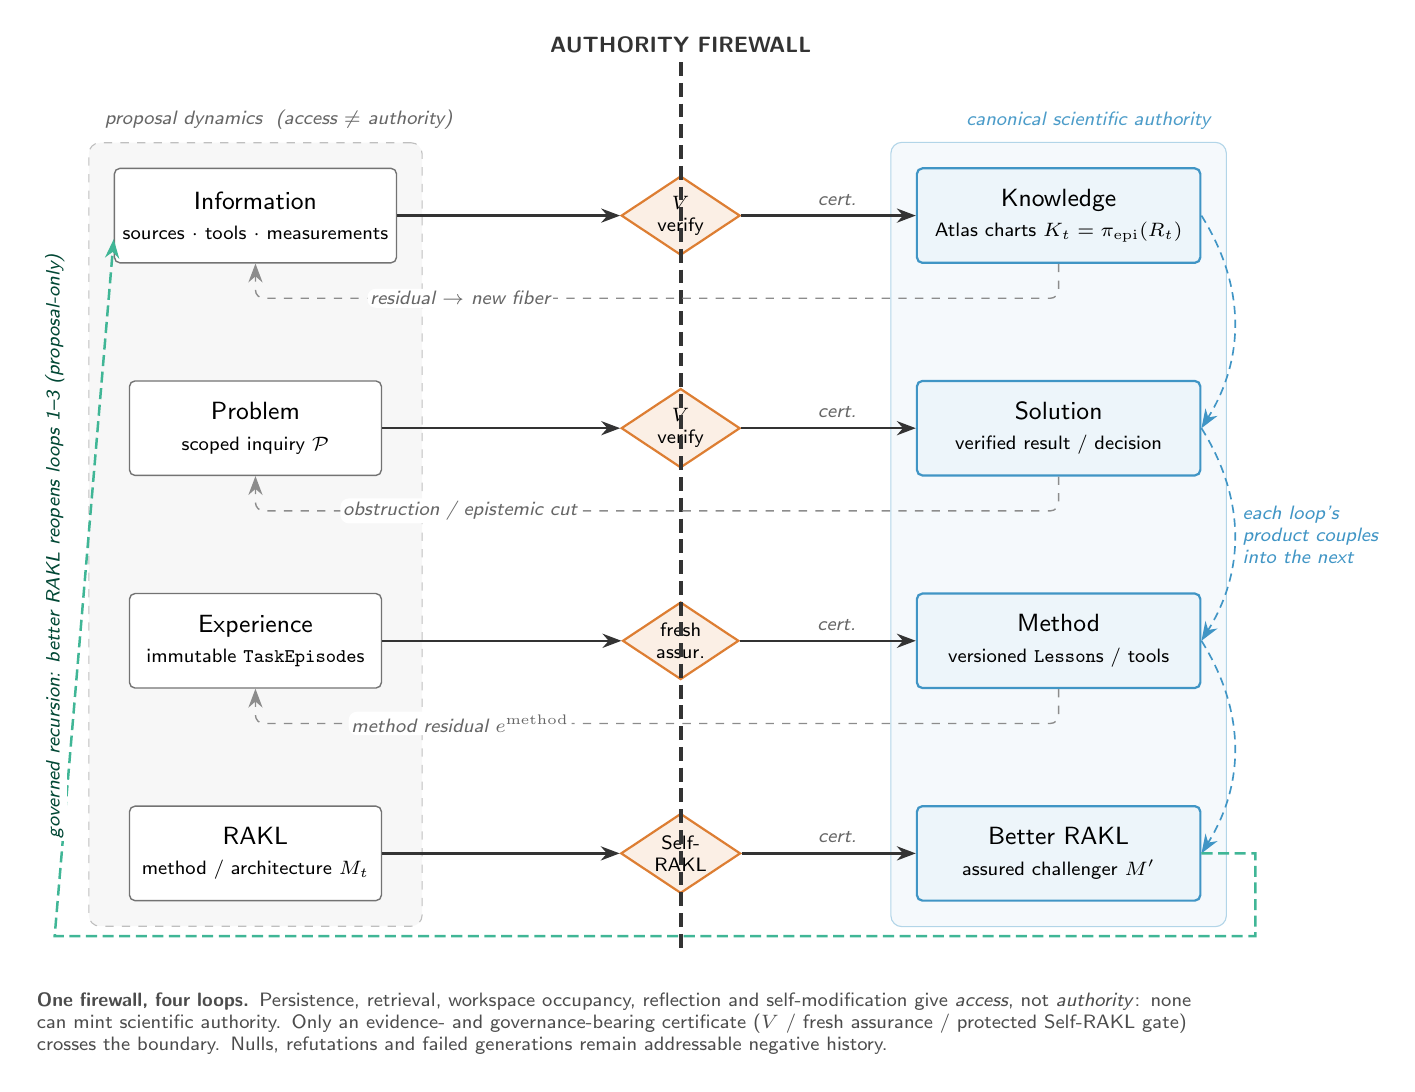
\begin{tikzpicture}[
  font=\small,
  >={Stealth[length=2.4mm]},
  loopin/.style={rounded corners=2pt, draw=black!55, line width=0.5pt, align=center,
                 inner sep=3pt, minimum height=12mm, minimum width=32mm, fill=white},
  loopout/.style={loopin, draw=oiblue!75, fill=oiblue!7, line width=0.8pt, minimum width=36mm},
  gatenode/.style={diamond, aspect=1.5, draw=oiverm!80, line width=0.8pt, fill=oiverm!10,
                   align=center, inner sep=1pt, font=\scriptsize},
  fwd/.style={->, line width=0.85pt, draw=black!80},
  ret/.style={->, line width=0.5pt, draw=black!45, dashed},
  couple/.style={->, line width=0.6pt, draw=oiblue!75, dash pattern=on 3pt off 2pt},
  reco/.style={->, line width=0.9pt, draw=oigreen!75, dash pattern=on 4pt off 2pt},
  lbl/.style={font=\scriptsize\itshape, text=black!60},
]
% ---- row y-positions ----
\def\ry{2.7}   % row spacing (cm)
% left inputs (x=0), gates (x=5.4), right outputs (x=10.2)
\node[loopin]  (in1) at (0, 0)         {Information\\{\scriptsize sources $\cdot$ tools $\cdot$ measurements}};
\node[loopin]  (in2) at (0,-\ry)       {Problem\\{\scriptsize scoped inquiry $\mathcal P$}};
\node[loopin]  (in3) at (0,-2*\ry)     {Experience\\{\scriptsize immutable \texttt{TaskEpisode}s}};
\node[loopin]  (in4) at (0,-3*\ry)     {RAKL\\{\scriptsize method / architecture $M_t$}};

\node[gatenode] (g1) at (5.4, 0)       {$V$\\verify};
\node[gatenode] (g2) at (5.4,-\ry)     {$V$\\verify};
\node[gatenode] (g3) at (5.4,-2*\ry)   {fresh\\assur.};
\node[gatenode] (g4) at (5.4,-3*\ry)   {Self-\\RAKL};

\node[loopout] (ot1) at (10.2, 0)      {Knowledge\\{\scriptsize Atlas charts $K_t=\pi_{\mathrm{epi}}(R_t)$}};
\node[loopout] (ot2) at (10.2,-\ry)    {Solution\\{\scriptsize verified result / decision}};
\node[loopout] (ot3) at (10.2,-2*\ry)  {Method\\{\scriptsize versioned \texttt{Lesson}s / tools}};
\node[loopout] (ot4) at (10.2,-3*\ry)  {Better RAKL\\{\scriptsize assured challenger $M'$}};

% ---- background panels ----
\begin{scope}[on background layer]
  \node[draw=black!25, dashed, rounded corners=4pt, fill=black!3,
        fit=(in1)(in4), inner sep=9pt] (lpanel) {};
  \node[draw=oiblue!30, rounded corners=4pt, fill=oiblue!4,
        fit=(ot1)(ot4), inner sep=9pt] (rpanel) {};
\end{scope}
\node[lbl, anchor=south west] at ([yshift=1pt]lpanel.north west)
      {\ proposal dynamics \ (access $\neq$ authority)};
\node[lbl, anchor=south east, text=oiblue!70] at ([yshift=1pt]rpanel.north east)
      {canonical scientific authority \ };

% ---- authority firewall (single bold boundary crossing all four loops) ----
\coordinate (ftop) at (5.4, 1.95);
\coordinate (fbot) at (5.4,-9.35);
\draw[line width=1.5pt, black!80, dash pattern=on 5pt off 2.5pt] (ftop) -- (fbot);
\node[anchor=south, font=\footnotesize\bfseries, text=black!80] at (ftop)
      {AUTHORITY FIREWALL};

% ---- forward flows (proposal -> gate -> licensed update) ----
\foreach \i in {1,2,3,4}{
  \draw[fwd] (in\i) -- (g\i);
  \draw[fwd] (g\i) -- node[lbl,above,pos=0.55]{\scriptsize cert.} (ot\i);
}
% ---- per-loop return: residual reopens the loop (proposal-only), routed cleanly below each row ----
\begin{scope}[rounded corners=3pt]
\draw[ret] (ot1.south) -- (10.2,-1.05) -- (0,-1.05) -- (in1.south);
\node[lbl, fill=white, inner sep=1pt] at (2.6,-1.05) {residual $\to$ new fiber};
\draw[ret] (ot2.south) -- (10.2,-3.75) -- (0,-3.75) -- (in2.south);
\node[lbl, fill=white, inner sep=1pt] at (2.6,-3.75) {obstruction / epistemic cut};
\draw[ret] (ot3.south) -- (10.2,-6.45) -- (0,-6.45) -- (in3.south);
\node[lbl, fill=white, inner sep=1pt] at (2.6,-6.45) {method residual $e^{\mathrm{method}}$};
\end{scope}

% ---- inter-loop coupling: each loop's product conditions the next (far right) ----
\draw[couple] (ot1.east) to[bend left=32] (ot2.east);
\draw[couple] (ot2.east) to[bend left=32] (ot3.east);
\draw[couple] (ot3.east) to[bend left=32] (ot4.east);
\node[lbl, text=oiblue!75, anchor=west, align=left] at ([xshift=4mm]$(ot2.east)!0.5!(ot3.east)$)
      {each loop's\\product couples\\into the next};

% ---- fourth loop / governed recursion: better RAKL reopens loops 1-3 ----
\draw[reco] (ot4.east) -- (12.7,-8.1) -- (12.7,-9.15) -- (-2.55,-9.15) -- ([yshift=-3mm]in1.west);
\node[lbl, text=oigreen!45!black, rotate=90, fill=white, inner sep=1pt] at (-2.55,-4.2)
      {governed recursion: better RAKL reopens loops 1--3 (proposal-only)};

% ---- forbidden-coercion note ----
\node[anchor=north west, font=\scriptsize, text width=150mm, align=left, black!70]
      at (-2.9,-9.75)
      {\textbf{One firewall, four loops.} Persistence, retrieval, workspace occupancy, reflection and
       self-modification give \emph{access}, not \emph{authority}: none can mint scientific authority.
       Only an evidence- and governance-bearing certificate ($V$ / fresh assurance / protected Self-RAKL gate)
       crosses the boundary. Nulls, refutations and failed generations remain addressable negative history.};
\end{tikzpicture}
\end{document}
